% !TEX program = xelatex
\documentclass[12pt,a4paper,oneside]{report}
\usepackage[T1]{fontenc}
\usepackage{lmodern}
\usepackage[a4paper,left=28mm,right=25mm,top=25mm,bottom=25mm,headheight=15pt]{geometry}
\usepackage{amsmath,amssymb,graphicx,booktabs,tabularx,array,multirow}
\usepackage{xcolor,setspace,fancyhdr,titlesec,caption,subcaption,enumitem}
\usepackage{tikz}
\usetikzlibrary{arrows.meta,positioning,shapes.geometric,calc}
\usepackage{microtype}
\usepackage{placeins,float}
\usepackage[numbers,sort&compress]{natbib}
\usepackage[hidelinks,bookmarksnumbered,hypertexnames=false,pdfauthor={Lakshay Gupta},pdftitle={GenoPred Multi Omic Learning for Pancreatic Cancer Driver Gene Prioritization}]{hyperref}
\usepackage{bookmark}
\makeatletter
\let\tableinput\@@input
\makeatother
\definecolor{navy}{HTML}{19344B}
\definecolor{teal}{HTML}{167D9A}
\definecolor{pale}{HTML}{EEF4F7}
\setstretch{1.18}
\setlength{\parindent}{1.2em}
\setlength{\parskip}{4pt}
\setlength{\emergencystretch}{2em}
\raggedbottom
\brokenpenalty=10000
\clubpenalty=10000
\widowpenalty=10000
\setcounter{tocdepth}{1}
\setcounter{secnumdepth}{2}
\captionsetup{font=small,labelfont=bf,labelsep=period,skip=8pt}
\captionsetup[table]{position=top}
\setlist{itemsep=3pt,topsep=5pt,leftmargin=1.6em}
\renewcommand{\arraystretch}{1.22}
\newcolumntype{Y}{>{\raggedright\arraybackslash}X}
\newcommand{\roi}{\ensuremath{96\times96\times96}}
\newcommand{\model}{\textsc{CompactResNet3D}}
\newcommand{\note}[1]{\par\smallskip\noindent\colorbox{pale}{\parbox{\dimexpr\linewidth-2\fboxsep\relax}{\small #1}}\par\smallskip}
\titleformat{\chapter}[display]{\normalfont\bfseries\color{navy}}{\large\MakeUppercase{\chaptertitlename}\ \thechapter}{8pt}{\huge}
\titlespacing*{\chapter}{0pt}{-14pt}{23pt}
\titleformat{\section}{\normalfont\large\bfseries\color{navy}}{\thesection}{.7em}{}
\titleformat{\subsection}{\normalfont\normalsize\bfseries}{\thesubsection}{.7em}{}
\pagestyle{fancy}
\fancyhf{}
\fancyhead[L]{\small\nouppercase{\leftmark}}
\fancyfoot[C]{\thepage}
\renewcommand{\headrulewidth}{0.35pt}
\renewcommand{\chaptermark}[1]{\markboth{\thechapter.\ #1}{}}
\fancypagestyle{plain}{\fancyhf{}\fancyfoot[C]{\thepage}\renewcommand{\headrulewidth}{0pt}}
\graphicspath{{images/}}
\begin{document}
\begin{titlepage}
\centering
\vspace*{6mm}
{\Large\bfseries GenoPred Multi Omic Learning for\\[5pt] Pancreatic Cancer Driver Gene Prioritization\par}
\vspace{10mm}
{\large B.Tech Project I\par}
\vspace{5mm}
{A report submitted in partial fulfilment of the requirements\\for the degree of\par}
\vspace{4mm}
{\large\bfseries Bachelor of Technology\\in Chemical Engineering\par}
\vspace{11mm}
{Submitted by\par}
{\large\bfseries Lakshay Gupta\par}
{Roll No. 23CH10037\par}
\vspace{9mm}
{Under the supervision of\par}
{\large\bfseries Prof. Nikita Saxena\par}
{Department of Chemical Engineering\par}
\vspace{10mm}

\includegraphics[height=30mm]{iit_kharagpur.png}\par
\vspace{8mm}
{\bfseries Department of Chemical Engineering\\Indian Institute of Technology Kharagpur\par}
\vfill
{\small Review draft\par}
\end{titlepage}
\pagenumbering{roman}
\pagestyle{plain}
\chapter*{Declaration}
\addcontentsline{toc}{chapter}{Declaration}
I, Lakshay Gupta (Roll No. 23CH10037), submit this report entitled \emph{GenoPred Multi Omic Learning for Pancreatic Cancer Driver Gene Prioritization} as part of B.Tech Project I in the Department of Chemical Engineering, Indian Institute of Technology Kharagpur.

The report presents the implemented methods and recorded experiments in the GenoPred project materials. Public data, established methods and software sources are acknowledged. Completed experiments are distinguished from proposed extensions, and material implementation limitations are disclosed.

This declaration is provided for the student's review and signature before submission.
\vspace{26mm}
\begin{flushright}
\rule{54mm}{0.4pt}\\
Lakshay Gupta\\
Roll No. 23CH10037
\end{flushright}
\vspace{8mm}
\noindent Date: \rule{35mm}{0.4pt}

\chapter*{Certificate}
\addcontentsline{toc}{chapter}{Certificate}
This page is reserved for certification of the report entitled \emph{GenoPred Multi Omic Learning for Pancreatic Cancer Driver Gene Prioritization}, submitted by Lakshay Gupta (Roll No. 23CH10037) towards B.Tech Project I in the Department of Chemical Engineering, Indian Institute of Technology Kharagpur.

Certification is subject to the supervisor's review, approval and signature. No supervisor approval is implied by this unsigned draft.

\vspace{32mm}
\noindent\rule{65mm}{0.4pt}\\
\textbf{Prof. Nikita Saxena}\\
Department of Chemical Engineering\\
Indian Institute of Technology Kharagpur\\
Supervisor
\vspace{12mm}

\noindent Date: \rule{35mm}{0.4pt}

\chapter*{Abstract}\addcontentsline{toc}{chapter}{Abstract}
GenoPred develops a reproducible gene-level pipeline for prioritizing pancreatic cancer driver candidates from molecular features and protein-interaction data. The study integrates TCGA-PAAD mutation, copy-number and RNA measurements with patient and cell-line regulatory assays. The resulting dataset contains 19,962 protein-coding genes, ten biological features and ten missingness indicators. A conservative external evidence rule identifies 17 positive genes; the remaining 19,945 genes remain unlabelled rather than being asserted to be biological negatives.

Linear non-negative positive-unlabelled learning is compared with PU tree procedures, a mutation-prevalence baseline and exploratory network diffusion. Five repeats of three-fold outer gene-level evaluation, with three-fold inner model selection, give mean observed-label average precision of 0.5517 for nnPU, 0.5025 for mutation prevalence, 0.4490 for LightGBM, 0.3160 for gradient boosting and 0.1365 for a shallow tree. Repeated nested evaluation provides the primary internal comparison.

Separately tuned feature experiments give nnPU average precision of 0.5428 for mutation plus expression and 0.5517 for the full feature set. The full-feature advantage is modest and does not establish that every regulatory assay contributes useful information. Leave-one-positive-out experiments and candidate-stability analysis expose gene-specific failure modes and sensitivity to the available positive labels.

External assessments provide mixed evidence. Provisional MSK sequence-evidence labels and a source-reconciled autopsy assessment give dataset-dependent model rankings. CRISPR survival associations are small, with no top-100 enrichment for the shortlisted models. The combined results establish a working research pipeline with useful internal retrieval performance and measurable candidate stability. Evaluation remains exploratory because the positive-label set is small and independent biological validation is incomplete.

\vspace{3mm}\noindent\textbf{Keywords:} pancreatic cancer; driver-gene prioritization; multi-omic features; positive-unlabelled learning; nested evaluation; reproducibility.

\tableofcontents
\clearpage
\listoffigures
\addcontentsline{toc}{chapter}{List of Figures}
\clearpage
\listoftables
\addcontentsline{toc}{chapter}{List of Tables}
\clearpage
\chapter*{Abbreviations}
\addcontentsline{toc}{chapter}{Abbreviations}
\begin{tabularx}{\linewidth}{lY}
\toprule
AP & Average precision against observed positive labels\\
ATAC & Assay for transposase-accessible chromatin\\
AUROC & Area under the receiver operating characteristic curve\\
CNV & Copy-number variation\\
CPM & Counts per million\\
CRISPR & Clustered regularly interspaced short palindromic repeats\\
GDC & Genomic Data Commons\\
GEO & Gene Expression Omnibus\\
GRCh38 & Genome Reference Consortium human build 38\\
HGNC & HUGO Gene Nomenclature Committee\\
HPNE & Human pancreatic nestin-expressing cell model\\
ICGC & International Cancer Genome Consortium\\
LOPO & Leave-one-positive-out evaluation\\
MSK & Memorial Sloan Kettering\\
nnPU & Non-negative positive-unlabelled learning\\
OOF & Out-of-fold\\
PAAD & Pancreatic adenocarcinoma project designation\\
PDAC & Pancreatic ductal adenocarcinoma\\
PU & Positive-unlabelled\\
TCGA & The Cancer Genome Atlas\\
TPM & Transcripts per million\\
TSS & Transcription start site\\
\bottomrule
\end{tabularx}

\clearpage
\pagenumbering{arabic}
\pagestyle{fancy}
\fancyhf{}
\fancyhead[L]{\small\nouppercase{\leftmark}}
\fancyfoot[C]{\thepage}
\renewcommand{\headrulewidth}{0.35pt}
\chapter{Introduction}
\section{Motivation}
GenoPred is a B.Tech research project that develops a gene-level pancreatic cancer prioritization pipeline with models trained from scratch. A pancreatic tumour can contain many molecular alterations, but their presence alone does not establish a causal role in cancer development. Driver-gene prioritization seeks to order genes for further investigation by combining evidence about mutation, dosage, expression and regulation. GenoPred addresses this ranking problem at gene level, using patient measurements as inputs to gene summaries rather than predicting a patient diagnosis.

The central difficulty is incomplete biological knowledge. A small set of genes has replicated evidence, whereas most genes lack a definitive classification. Treating all remaining genes as negatives would turn absence of evidence into evidence of absence. The project therefore adopts a positive-unlabelled learning framework and reports recovery of observed evidence labels.

Reproducibility is also a scientific requirement. Coordinate mismatches, inconsistent identifiers or repeated patient libraries can distort apparently valid model inputs. GenoPred combines data harmonization, explicit missingness, conservative labels and saved evaluation artifacts so that ranking claims can be traced to the calculations that produced them.

\section{Problem definition}
For each gene g, a feature vector x(g) contains ten biological measurements and ten missing-value indicators. The observed label s(g) is positive for 17 genes and unlabelled for 19,945 genes. A scoring function f produces an ordering over the 19,962-gene universe. A high score identifies a candidate for review; it is not a calibrated probability of driver status.

The research question is how reliably pancreatic molecular features retrieve known and independently reported candidate genes, and how linear nnPU, tree methods and simple biological baselines compare under controlled gene-level evaluation. Patient-level survival prediction, diagnosis and treatment selection are outside this task.

\section{Objectives and contributions}
The first objective is to construct a coherent molecular dataset with aligned gene identifiers, declared genome coordinates and reproducible patient aggregation. The second is to define evidence labels without manufacturing reliable negatives. The third is to compare ranking procedures under training-partition preprocessing and validation-based model selection. The fourth is to examine agreement with external genomic and functional evidence while retaining their limitations.

The completed implementation provides immutable source inventories, a 165-case TCGA cohort, a 40-patient accessibility summary, a finite 19,962-by-20 feature matrix and a high-confidence STRING physical-interaction graph. It implements linear nnPU, PU tree procedures and graph diffusion, followed by repeated internal evaluation, separately tuned feature comparisons and leave-one-positive-out assessment.

The project successfully integrates complementary molecular evidence into a reproducible ranking framework. Linear nnPU achieves the highest mean AP among the shortlisted procedures in repeated evaluation, improving on mutation prevalence alone. Independently tuned feature comparisons and gene-specific tests provide complementary evidence about candidate retrieval and stability.

\section{Organisation of the report}
Chapter 2 introduces incomplete labels, molecular evidence and the modelling framework. Chapter 3 describes source acquisition, harmonization and quality assurance. Chapter 4 explains the feature construction, model procedures and evaluation design. Chapter 5 reports the repeated internal results, feature-value experiments and external assessments. Chapter 6 discusses limitations, and Chapter 7 identifies the conclusions and priorities for continuation. Appendix A records reproducibility; Appendix B documents data-processing and model-verification procedures. References distinguish project records from primary method sources.

\chapter{Background and Related Work}
\section{Molecular evidence and driver prioritization}
Mutation prevalence describes the fraction of selected cases with a qualifying sequence alteration in a gene. Copy-number gain and loss provide complementary dosage information, while RNA abundance summarizes transcriptional activity. Regulatory assays describe accessibility or protein-associated signal near promoters. These measurements answer related but distinct questions and cannot be interpreted as interchangeable proof of driver activity.

GenoPred combines patient-derived measurements with PANC-1 and HPNE cell-model contrasts. The latter provide a controlled regulatory comparison, but HPNE is an immortalised comparison model and does not represent every normal pancreatic cell state. Cross-study differences and model-specific biology remain possible sources of variation. The implementation and source identifiers are documented in the Stage 3 and Stage 5 project records.

\section{Positive unlabelled learning}
Positive-unlabelled learning uses a labelled positive subset together with an unlabelled population that can contain both true classes. Non-negative PU risk estimation prevents the estimated negative-risk component from becoming arbitrarily negative during optimization. Kiryo and colleagues introduced this approach as a means of controlling overfitting in PU learning.~\cite{ref10}

GenoPred uses a linear scoring model with an assumed positive class prior. The observed labelled fraction is not automatically the true prevalence of driver genes. Conservative evidence selection also favours well-studied, detectable mechanisms, so the labelled positives need not be representative of all biologically relevant genes. This is a substantive limitation of the learning problem, not a numerical preprocessing issue.

\section{Interaction networks and model scope}
STRING supplies protein-interaction evidence that can be represented as a graph. The project selects the physical network at a fixed high-confidence threshold, rather than equating all functional associations with direct physical contact. STRING version 12 is described by Szklarczyk and colleagues.~\cite{ref11}

The implemented graph baseline is random-walk score diffusion. It combines neighbouring scores with a retained starting score; it is not a trained graph neural network. Breast-to-pancreas transfer learning, deep graph models and Hi-C-derived features remain proposed extensions rather than completed methods in this report.

\chapter{Dataset and Quality Assurance}
\section{Selected data and provenance}
The core acquisition comprises 561 verified files from TCGA-PAAD, GSE149103 and GSE124229~\cite{ref14,ref12,ref13}. Original files are kept separate from processed tables and are recorded with hashes and source metadata. A common harmonized feature dataset is used throughout the reported model comparisons.

\begin{table}[H]\centering
\caption{Core source inventory and role.}
{\small
\begin{tabularx}{\textwidth}{@{}>{\raggedright\arraybackslash}X>{\raggedright\arraybackslash}X>{\raggedright\arraybackslash}X@{}}\toprule
\textbf{Source} & \textbf{Files} & \textbf{Role}\\\midrule
TCGA-PAAD & 542 & RNA, masked somatic mutations and gene-level CNV\\
GSE149103 & 18 & PANC-1/HPNE regulatory tracks and acquired Hi-C archives\\
GSE124229 & 1 & Patient ATAC atlas count matrix\\
GENCODE v36 & Reference & Gene identity and canonical coordinates\\
IntOGen snapshot & Labels & Externally replicated pancreatic evidence\\
STRING v12.0 & Network & High-confidence physical interactions\\
\bottomrule\end{tabularx}}
\end{table}
The TCGA inventory contains 183 RNA files, 179 CNV files and 180 mutation files. Their case associations do not define identical cohorts. The canonical modelling subset comprises 165 primary-tumour cases with all three required modalities. Accessibility is summarized separately from 80 assay libraries representing 40 patient identifiers.

\section{Gene identities and coordinates}
GENCODE v36 supplies 60,660 assembly gene records; the label and model universe is restricted to 19,962 protein-coding genes. Deterministic node indices align the feature matrix, labels and graph. Ambiguous symbol mappings are excluded rather than arbitrarily assigned. GRCh38 is the canonical coordinate system; hg19 GEO inputs pass an explicit harmonization route before feature extraction.

\section{Harmonization and assay quality assurance}
After liftover to GRCh38, the patient ATAC atlas retains 119,299 of 119,466 intervals (99.860\%) and 98.442\% of signal mass. Retention measures coordinate transformation, not biological relevance. All 16 GSE149103 bigWigs have consistent hg19 chromosome sizes.

Promoter windows extend 2 kb on each side of the TSS. Reverse liftover maps canonical coordinates to hg19 signal tracks. Unique mappings must preserve orientation and a length ratio of 0.8--1.25. Interior checks every 100 bp reject excessive displacement; unavailable windows are missing.

Patient accessibility replicates are combined before between-patient summaries are calculated. Treating 80 libraries as 80 independent patients would exaggerate the apparent replication. TCGA mutation prevalence counts a case once per gene even if several qualifying variant rows occur in that case. These rules preserve the intended observational unit.

\section{Positive evidence and unknown genes}
\begin{table}[H]\centering
\caption{Gene universe and fixed experimental partition.}
{\small
\begin{tabularx}{\textwidth}{@{}>{\raggedright\arraybackslash}X>{\raggedright\arraybackslash}X>{\raggedright\arraybackslash}X>{\raggedright\arraybackslash}X@{}}\toprule
\textbf{Partition} & \textbf{Positive} & \textbf{Unlabelled} & \textbf{Total}\\\midrule
Training & 11 & 11,967 & 11,978\\
Validation & 3 & 3,989 & 3,992\\
Test & 3 & 3,989 & 3,992\\
All genes & 17 & 19,945 & 19,962\\
\bottomrule\end{tabularx}}
\end{table}
Positive labels require pancreatic evidence from at least two independent study families among CPTAC, ICGC PACA-AU and ICGC PACA-CA. Multiple analyses from one family count once. The pinned IntOGen snapshot yields 17 positives and 19,945 unlabelled genes, with no reliable-negative class.

TCGA is excluded from labels because mutation prevalence is an input. PCAWG is supporting-only because of ICGC donor overlap. CPTAC and ICGC supply labels, not untouched validation. This reduces direct circularity but cannot eliminate shared-knowledge or annotation bias.

\chapter[Methodology and Experimental Design]{Methodology and Experimental\\Design}
\section{Feature construction and missingness}
Each gene receives ten biological values and one missingness flag per value. Storage-time imputation only creates a finite matrix. During modelling, the flags recover unavailable entries and medians are refitted using the permitted training genes; scaling is likewise fitted inside the relevant training partition. Thus the stored global placeholders do not determine test-fold preprocessing.

\begin{table}[H]\centering
\caption{Implemented biological features.}
{\small
\begin{tabularx}{\textwidth}{@{}>{\raggedright\arraybackslash}X>{\raggedright\arraybackslash}X@{}}\toprule
\textbf{Feature group} & \textbf{Definition}\\\midrule
Cell-line ATAC & Difference of replicate-median log1p promoter signal\\
Cell-line CTCF, H3K4me3, H3K27ac & Three differences of replicate-median signed promoter signals\\
Patient ATAC mean & 10\% trimmed mean of 40 patient log1p(CPM) profiles\\
Patient ATAC variability & Median absolute deviation across those patient profiles\\
Mutation prevalence & Cases with selected damaging consequences divided by 165\\
Amplification prevalence & Fraction with CNV at least twice the case modal baseline\\
Deletion prevalence & Fraction below the case modal baseline, including zero\\
Tumour expression & Median log2(TPM + 1) over the 165 cases\\
\bottomrule\end{tabularx}}
\end{table}
The autosomal CNV baseline is estimated separately for each case, taking the larger mode in a tie. Sex-chromosome CNV is missing until a validated sex-aware calculation is available. A total of 953 genes have unavailable CNV values. Gene-specific exome callability masks were unavailable; the mutation denominator remains the selected 165-case cohort.

Hi-C features are deferred. CRISPR dependency measurements are reserved for functional assessment and do not enter the training feature matrix. This separation prevents a later functional comparison from merely recovering a measurement already supplied to the model.

\section{Linear nnPU and graph diffusion}
For standardized features x, the linear model forms a score from a weighted sum and an intercept. The logistic output provides a bounded ranking score. Its coefficients describe model associations; neither coefficients nor scores establish causal gene effects. The fitted bundle stores feature order, imputation, scaling, weights and intercept.

The nnPU objective combines a positive loss term with the non-negative part of the estimated unlabelled-minus-positive negative loss. In compact notation, its risk has the form below, with an additional L2 penalty on the weights. The class prior pi is assumed and selected from a declared grid.~\cite{ref10}

\begin{equation}R_{\mathrm{nnPU}}=\pi R_P^{+}+\max\{0,R_U^{-}-\pi R_P^{-}\}+\lambda\lVert w\rVert^2.\end{equation}
Here RP denotes an empirical average over labelled positives, RU an average over unlabelled genes, and the signs identify the assumed class for the loss. GenoPred uses a linear model rather than the flexible deep architectures also possible within the general PU framework.

The STRING graph contains 85,171 distinct undirected interactions, stored as 170,342 directed entries. At confidence score 700 or above, 10,599 genes are connected and 9,363 are isolated. Self-loops preserve a valid transition for every gene. Weighted random-walk diffusion blends neighbour information with the original feature-model score; the exploratory fixed-split experiment selects restart 0.5 from 0.3, 0.5, 0.7 and 0.9.

This graph setting is transductive: the full topology is available while test labels are withheld from fitting. An isolated gene retains its own score, although its rank can change when other genes move. The positive gene LRP1B is isolated under the fixed threshold, which was not relaxed to force connectivity.

\section{PU tree procedures and baseline controls}
PU bagging repeatedly samples unlabelled genes to form temporary comparator sets and aggregates the fitted learners. These sampled genes are not declared reliable biological negatives. Shallow decision trees, gradient boosting and LightGBM provide nonlinear alternatives to the linear nnPU procedure. The final repeated comparison uses six bags per fit and ten sampled unlabelled genes per training positive.

Mutation prevalence is an essential biological baseline. Feature ablations, missingness-only models and shuffled labels provide diagnostics of what the model learns. A complex learner must be compared with this baseline before its performance can be attributed to multi-omic integration.

\section{Repeated nested gene level evaluation}
The primary internal evaluation uses five fixed random seeds, each defining three stratified outer folds. Each gene appears in the test partition exactly once per repeat. An outer test fold contains five or six positives and approximately 6,650 genes overall. Within each outer training set, three inner folds select settings using mean observed-label AP.

Missing-value replacement and scaling are fitted only on the current training partition. Outer test labels and features do not participate in fitting or hyperparameter selection. After inner selection, the chosen procedure is refitted on the outer training genes and evaluated on the outer test genes. This assesses the complete training and selection procedure.

\begin{table}[H]\centering
\caption{Repeated evaluation and sensitivity settings.}
{\small
\begin{tabularx}{\textwidth}{@{}>{\raggedright\arraybackslash}X>{\raggedright\arraybackslash}X@{}}\toprule
\textbf{Component} & \textbf{Recorded design}\\\midrule
Outer evaluation & 5 repeats $\times$ 3 stratified folds\\
Inner model selection & 3 folds within each outer training partition\\
nnPU grid & Priors 0.001, 0.003, 0.01; L2 0.0001, 0.01; 600 epochs\\
Tree-family grid & Depth 2 or 3; 6 PU bags; 10 sampled unlabelled per positive\\
Feature extension & Four feature groups independently tuned per learner\\
LOPO extension & 17 positive deletions; fixed 1,995 held-out unlabelled genes\\
Prior sensitivity & 5 priors $\times$ 2 feature sets $\times$ 3 folds in the first repeat\\
\bottomrule\end{tabularx}}
\end{table}
Metrics are averaged over three outer folds within a repeat and then across five repeats. The reported repeat range is descriptive, not a confidence interval: repeats share the same genes, evidence labels and feature sources. Model-family selection involved exploratory screening within this project, so the repeated analysis remains retrospective robustness evidence.

\section{Metrics and tied scores}
Observed-label AP summarizes precision at score thresholds where known positives are retrieved. Unlabelled comparators are not confirmed negatives, so AP is not biological precision or diagnostic accuracy. AUROC describes broad separation of observed labels but can obscure the quality of the top-ranked shortlist when positives are rare.

Top-k recall measures the fraction of known positives retrieved within the stated evaluation universe. At tied cutoffs, fractional credit avoids arbitrary identifier ordering. AP groups tied scores at common thresholds and displayed gene ranks use midranks. Top 100 in an outer test fold is not the top 100 of the full gene universe.

\section{Feature value and individual positive sensitivity}
The extension independently tunes four feature sets for nnPU, gradient boosting and LightGBM: mutation only, mutation plus CNV, mutation plus expression, and all features. Each biological group includes its associated missingness indicators. The same outer partitions support paired descriptive comparisons, while each group selects its own settings within training folds.

LOPO removes each of the 17 positives completely from training instead of relabelling it as unlabelled. Each fit uses the other 16 positives and 17,950 unlabelled genes; its test contains the omitted positive and the same 1,995 held-out unlabelled genes. Three-fold inner selection is repeated. The four procedures are full nnPU, mutation-only nnPU, full gradient boosting and full LightGBM.

Candidate stability compares the top-100 selections among those 1,995 held-out unlabelled genes across positive-deletion fits. Boundary ties receive weights whose total is exactly 100. Weighted Jaccard is the sum of pairwise minimum weights divided by the sum of pairwise maximum weights. This measures sensitivity to available positive examples and induced tuning, not whole-genome or cohort-shift stability.

Prior sensitivity fixes each of five nnPU priors, from 0.0005 to 0.03, and independently tunes L2 inside the first repeat's outer training folds. These are sensitivity diagnostics. Their outer results do not select a new production prior or establish the true fraction of hidden drivers.

\clearpage\section{External endpoints and implementation checks}
Frozen model predictions are assessed against three distinct endpoints: provisional recurrent sequence evidence in the MSK panel, a reconciled author-selected autopsy sequence set, and CRISPR cancer-cell survival measurements. Their gene universes and positive definitions differ; absolute AP values are therefore not directly comparable across endpoints.

Saved manifests retain source hashes, fold assignments, selection records and fitted bundles. The final extension record reports 64 passing tests and exact prediction reproduction from 248 saved bundles. These checks support execution consistency, but do not establish biological truth. Full-cohort feature aggregation precedes gene splitting, so the evaluation does not simulate an independent new patient cohort.

\chapter{Results}
\section{Primary repeated internal comparison}
Linear nnPU has the highest mean observed-label AP among the shortlisted procedures in repeated nested evaluation. Its mean AP is 0.5517, compared with 0.5025 for mutation prevalence. The mean difference is 0.0492 and is positive in all five repeat means. The point estimates describe this retrospective gene-level study and do not establish a universally best model.

\begin{table}[H]\centering
\caption{Repeated nested results with 17 positives over 19,962 genes. Top-k is within each outer test fold.}
{\small
\begin{tabularx}{\textwidth}{@{}>{\raggedright\arraybackslash}X>{\raggedright\arraybackslash}X>{\raggedright\arraybackslash}X>{\raggedright\arraybackslash}X>{\raggedright\arraybackslash}X@{}}\toprule
\textbf{Model} & \textbf{Mean observed-label AP} & \textbf{Range of repeat means} & \textbf{Mean top-100 recall} & \textbf{Mean top-500 recall}\\\midrule
nnPU & 0.5517 & 0.5350--0.5684 & 78.4\% & 85.6\%\\
LightGBM & 0.4490 & 0.3131--0.5339 & 71.6\% & 80.9\%\\
Gradient boosting & 0.3160 & 0.2145--0.4233 & 64.9\% & 75.1\%\\
Shallow tree & 0.1365 & 0.0278--0.2673 & 54.5\% & 64.0\%\\
Mutation baseline & 0.5025 & 0.4884--0.5193 & 77.0\% & 85.2\%\\
\bottomrule\end{tabularx}}
\end{table}
LightGBM is the strongest nonlinear alternative by mean AP in this comparison. The shallow tree has mean AP 0.1365 and a wide range across repeat means. Repeated evaluation therefore provides an informative basis for comparing the ranking procedures beyond one fixed partition.

The mutation baseline retains mean top-500 recall of 85.2\%, close to full nnPU at 85.6\%. Thus the numerical AP advantage should be considered alongside candidate recovery and the cost of the additional assays. Observed-label retrieval is the endpoint; the study has no verified negative gene set.

\section{Model comparison across evidence settings}
\begin{figure}[H]\centering
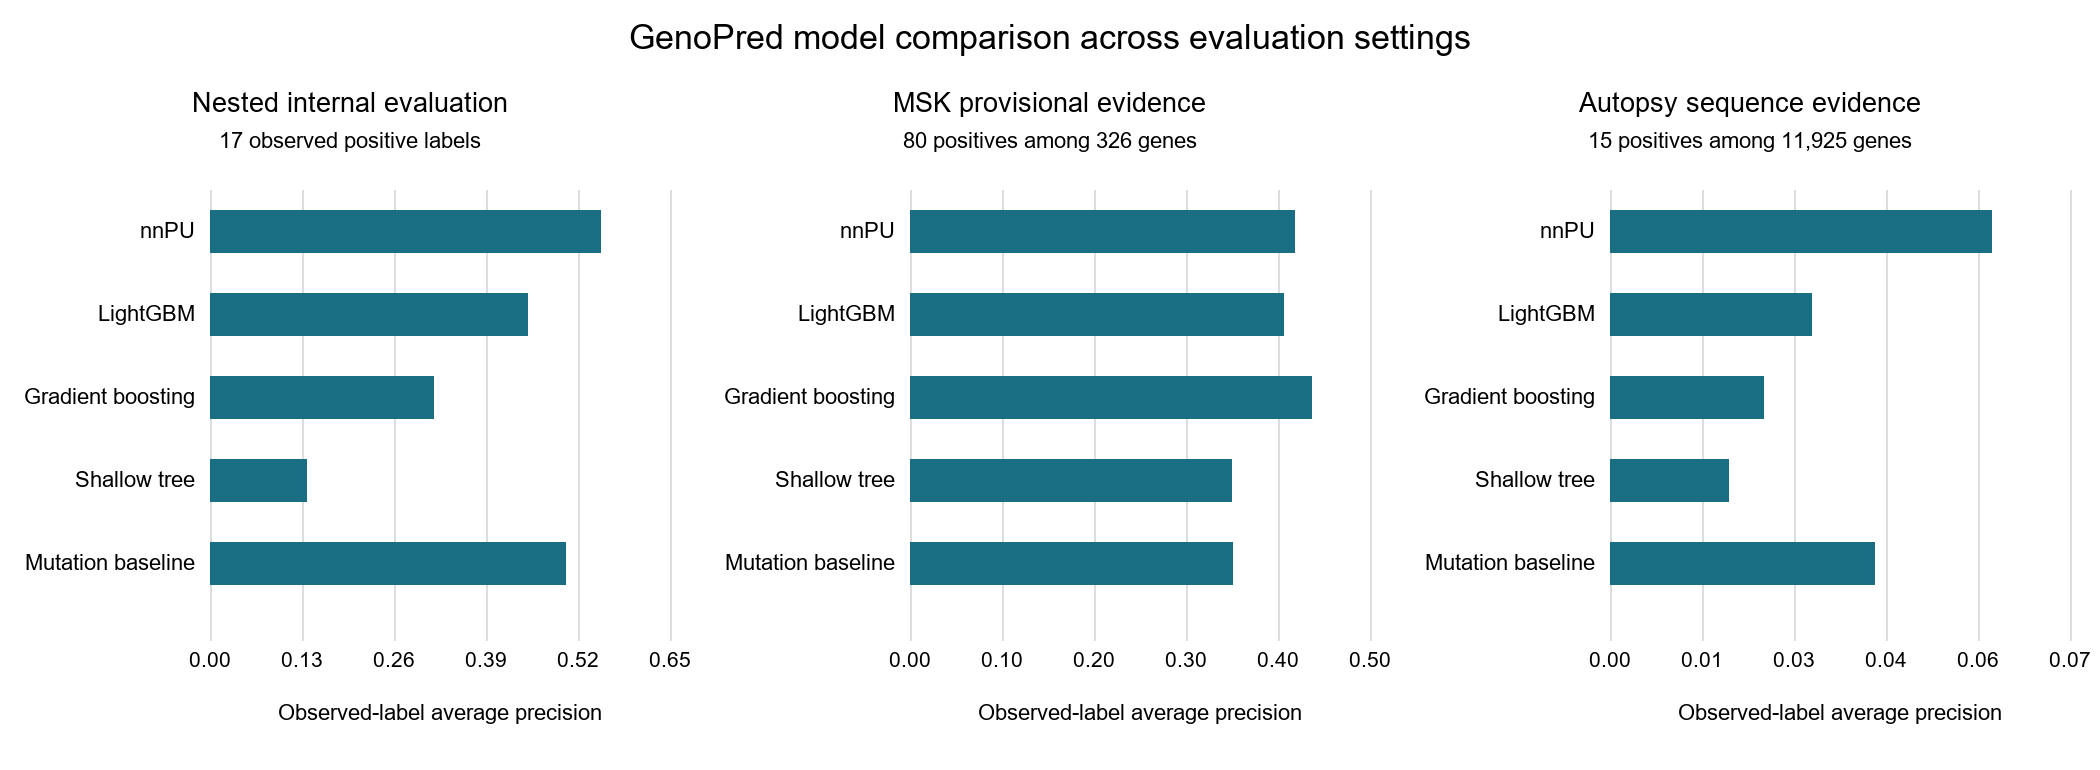
\includegraphics[width=\textwidth]{plot1.png}
\caption{Internal and external model comparisons. Each panel has its own gene universe, evidence prevalence and axis scale.}
\end{figure}
The internal panel summarizes repeated gene-level evaluation, whereas the external panels assess frozen predictions against different evidence sets. Model ordering depends on the endpoint: nnPU leads the repeated internal comparison and the small autopsy assessment, while gradient boosting has the highest provisional MSK AP point estimate.

The figure does not support comparison of absolute AP between panels. The MSK panel universe is much more enriched for provisional evidence labels than the genome-scale internal or autopsy universes. No paired superiority test identifies an externally validated winner.

\section{Fixed setting ablations}
\begin{table}[H]\centering
\caption{Fixed-setting ablations and controls in repeated internal evaluation.}
{\small
\begin{tabularx}{\textwidth}{@{}>{\raggedright\arraybackslash}X>{\raggedright\arraybackslash}X>{\raggedright\arraybackslash}X@{}}\toprule
\textbf{Diagnostic} & \textbf{nnPU mean AP} & \textbf{Gradient boosting mean AP}\\\midrule
Full features & 0.5517 & 0.3160\\
Without mutation & 0.0142 & 0.0016\\
Expression only & 0.0016 & 0.0012\\
Missingness only & 0.0010 & 0.0010\\
Shuffled labels & 0.0125 & 0.0018\\
\bottomrule\end{tabularx}}
\end{table}
Removing mutation prevalence and its flag sharply reduces AP. These ablations reuse settings selected for the full model, so they diagnose dependence under fixed settings rather than optimal performance of a reduced feature set. Separately tuned comparisons address that distinction next.

\section{Separately tuned feature combinations}
\begin{table}[H]\centering
\caption{Independently tuned feature sets. Means use five repeats; ranges are repeat means, not confidence intervals.}
{\small
\begin{tabularx}{\textwidth}{@{}>{\raggedright\arraybackslash}X>{\raggedright\arraybackslash}X>{\raggedright\arraybackslash}X>{\raggedright\arraybackslash}X>{\raggedright\arraybackslash}X@{}}\toprule
\textbf{Model} & \textbf{Features} & \textbf{Mean AP} & \textbf{Range of repeat means} & \textbf{Mean top-100 recall}\\\midrule
Gradient boosting & Full features & 0.3322 & 0.2145--0.4411 & 66.0\%\\
Gradient boosting & Mutation only & 0.2856 & 0.2489--0.3199 & 72.6\%\\
Gradient boosting & Mutation + CNV & 0.2520 & 0.2028--0.3437 & 68.0\%\\
Gradient boosting & Mutation + expression & 0.4501 & 0.3570--0.5081 & 68.2\%\\
LightGBM & Full features & 0.4595 & 0.3131--0.5367 & 71.6\%\\
LightGBM & Mutation only & 0.2731 & 0.2172--0.3206 & 76.9\%\\
LightGBM & Mutation + CNV & 0.2901 & 0.2666--0.3023 & 77.3\%\\
LightGBM & Mutation + expression & 0.4364 & 0.2674--0.5406 & 76.9\%\\
nnPU & Full features & 0.5517 & 0.5350--0.5684 & 78.4\%\\
nnPU & Mutation only & 0.5025 & 0.4884--0.5193 & 77.0\%\\
nnPU & Mutation + CNV & 0.5163 & 0.4998--0.5243 & 76.0\%\\
nnPU & Mutation + expression & 0.5428 & 0.5067--0.5594 & 82.0\%\\
\bottomrule\end{tabularx}}
\end{table}
For nnPU, mutation plus expression reaches AP 0.5428, compared with 0.5517 for all features. The full-feature increment over mutation plus expression is only 0.0089 and is positive in three repeat means but negative in two. Mutation plus expression has higher mean top-100 and top-500 recall, at 82.0\% and 88.0\%, than full nnPU at 78.4\% and 85.6\%.

The full feature set improves nnPU AP over mutation-only learning by 0.0492, but that observation does not show that each regulatory assay contributes independently. The simpler mutation-plus-expression model is a strong alternative when candidate recovery is the objective. Stochastic inner-fit seeds can also affect small differences between tree-model experiments.

\section{Leave one positive out assessment}
\begin{table}[H]\centering
\caption{LOPO results. Each test contains one omitted positive and 1,995 fixed unlabelled comparators.}
{\small
\begin{tabularx}{\textwidth}{@{}>{\raggedright\arraybackslash}X>{\raggedright\arraybackslash}X>{\raggedright\arraybackslash}X>{\raggedright\arraybackslash}X>{\raggedright\arraybackslash}X@{}}\toprule
\textbf{Model / features} & \textbf{Median positive rank} & \textbf{Mean single-positive AP} & \textbf{Top-100 credit} & \textbf{Top-500 credit}\\\midrule
Gradient boosting / Full features & 1.0 & 0.5969 & 76.5\% & 82.4\%\\
LightGBM / Full features & 1.0 & 0.6595 & 82.4\% & 88.2\%\\
nnPU / Full features & 3.0 & 0.5021 & 82.4\% & 94.1\%\\
nnPU / Mutation only & 3.5 & 0.4243 & 83.1\% & 94.6\%\\
\bottomrule\end{tabularx}}
\end{table}
\begin{table}[H]\centering
\caption{Held-out positive ranks within the 1,996-gene LOPO tests.}
{\small
\begin{tabularx}{\textwidth}{@{}>{\raggedright\arraybackslash}X>{\raggedright\arraybackslash}X>{\raggedright\arraybackslash}X>{\raggedright\arraybackslash}X>{\raggedright\arraybackslash}X@{}}\toprule
\textbf{Held-out gene} & \textbf{nnPU mutation rank} & \textbf{nnPU full rank} & \textbf{Gradient boosting full rank} & \textbf{LightGBM full rank}\\\midrule
CDKN2A & 1.0 & 1.0 & 1.0 & 1.0\\
SMAD4 & 1.0 & 1.0 & 1.0 & 1.0\\
TGFBR2 & 1.5 & 1.0 & 1.0 & 1.0\\
KRAS & 1.0 & 1.0 & 114.0 & 7.0\\
RNF43 & 1.0 & 1.0 & 1.0 & 1.0\\
TP53 & 1.0 & 1.0 & 1.0 & 1.0\\
KDM6A & 3.5 & 2.0 & 1.0 & 1.0\\
ARID1A & 2.5 & 2.0 & 1.0 & 1.0\\
KMT2D & 3.5 & 3.0 & 1.0 & 1.0\\
KMT2C & 3.5 & 3.0 & 1.0 & 1.0\\
ATM & 3.5 & 3.0 & 1.0 & 1.0\\
RBM10 & 6.5 & 4.0 & 10.0 & 1.0\\
LRP1B & 3.5 & 4.0 & 96.0 & 23.0\\
FAT1 & 54.5 & 45.0 & 41.0 & 50.0\\
SMARCA4 & 223.5 & 155.0 & 649.5 & 622.0\\
ACVR2A & 223.5 & 168.0 & 625.0 & 455.0\\
ACVR1B & 1179.5 & 1052.0 & 925.5 & 740.5\\
\bottomrule\end{tabularx}}
\end{table}
ACVR1B remains difficult for every procedure, while SMARCA4 and ACVR2A also expose sensitivity. With a single positive and no ties, AP equals reciprocal rank; tied thresholds and midranks require separate interpretation. These tests overlap heavily in training genes and are not independent biological replications.

\section{Candidate stability and prior sensitivity}
\begin{table}[H]\centering
\caption{Stability of top-100 selections among 1,995 held-out unlabelled genes.}
{\small
\begin{tabularx}{\textwidth}{@{}>{\raggedright\arraybackslash}X>{\raggedright\arraybackslash}X>{\raggedright\arraybackslash}X>{\raggedright\arraybackslash}X@{}}\toprule
\textbf{Model / features} & \textbf{Mean pairwise weighted Jaccard} & \textbf{Pairwise range} & \textbf{Genes fully selected in all 17 runs}\\\midrule
nnPU / full & 0.793 & 0.527--0.942 & 64\\
nnPU / mutation & 1.000 & 1.000--1.000 & 83\\
Gradient boosting / full & 0.659 & 0.205--0.961 & 15\\
LightGBM / full & 0.757 & 0.316--0.980 & 33\\
\bottomrule\end{tabularx}}
\end{table}
Full nnPU has mean weighted Jaccard 0.793 and 64 genes fully selected in all 17 fits. Mutation-only nnPU is unchanged across these positive deletions under the recorded fitting scheme. Stable selections can still reflect a consistent bias; stability is not correctness, and the analysis does not assess every gene in the model universe.

\begin{figure}[H]\centering
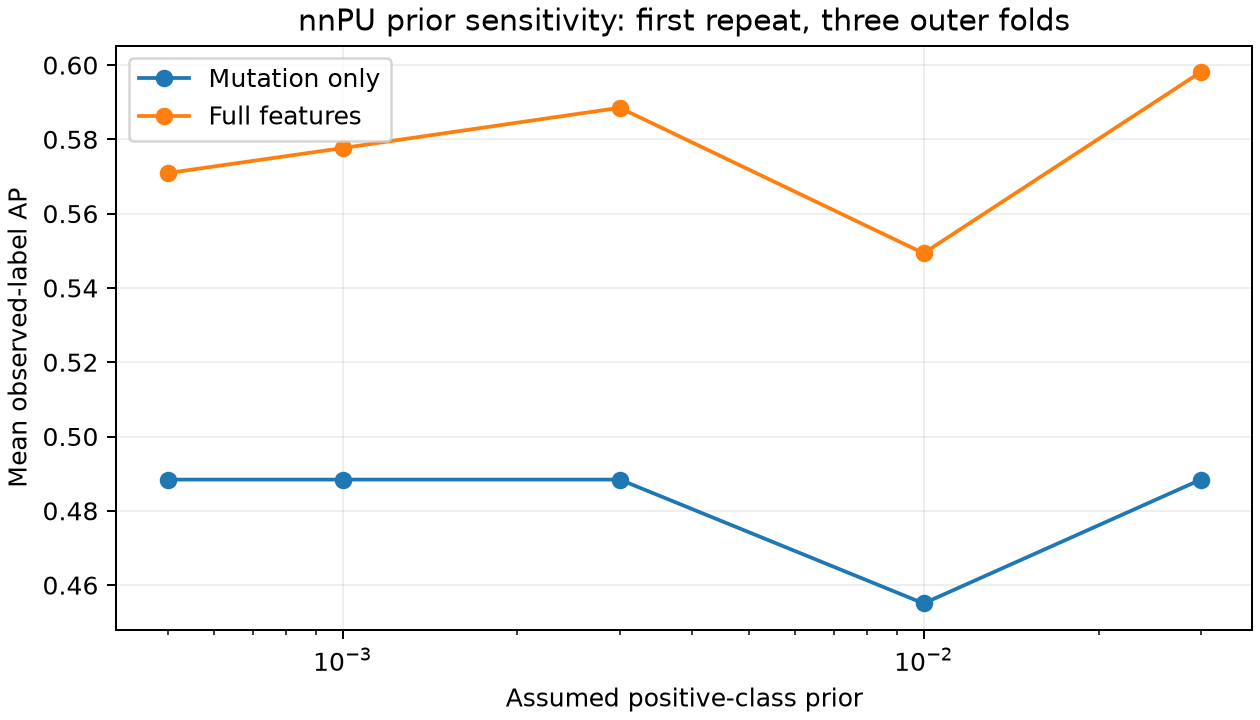
\includegraphics[width=\textwidth]{plot2.png}
\caption{Fixed-prior sensitivity in the first repeat. L2 is tuned separately for each prior and feature set.}
\end{figure}
Across the tested priors, full nnPU AP ranges from 0.5493 to 0.5981 in this three-fold diagnostic. The results quantify sensitivity to a modelling assumption; they do not estimate the biological prior or convert scores into calibrated probabilities.

\section{External genomic evidence}
\begin{table}[H]\centering
\caption{External comparisons. MSK: 326 genes and 80 provisional positives; autopsy: 11,925 genes and 15 positives; CRISPR: 15,767 eligible genes.}
{\small
\begin{tabularx}{\textwidth}{@{}>{\raggedright\arraybackslash}X>{\raggedright\arraybackslash}X>{\raggedright\arraybackslash}X>{\raggedright\arraybackslash}X>{\raggedright\arraybackslash}X>{\raggedright\arraybackslash}X@{}}\toprule
\textbf{Model} & \textbf{MSK AP} & \textbf{MSK top-100 recall} & \textbf{Autopsy AP} & \textbf{Autopsy top-500 recall} & \textbf{CRISPR correlation}\\\midrule
nnPU & 0.4179 & 47.5\% & 0.0581 & 53.3\% & 0.0229\\
LightGBM & 0.4056 & 41.2\% & 0.0306 & 53.3\% & 0.0695\\
Gradient boosting & 0.4365 & 42.5\% & 0.0234 & 40.0\% & 0.0504\\
Shallow tree & 0.3490 & 36.8\% & 0.0180 & 54.0\% & 0.0670\\
Mutation baseline & 0.3500 & 46.0\% & 0.0403 & 47.9\% & -0.0415\\
\bottomrule\end{tabularx}}
\end{table}
The MSK assessment starts from a published 2,336-patient dataset and restricts the evaluation to consistently assayed IMPACT341 genes with unique mappings, excluding the 17 training-label positives. Recurrent sequence alterations in at least three patients define 80 provisional evidence genes among 326 eligible genes. These are not 80 independently confirmed PDAC drivers.

Of 924 supporting sequence-alteration rows, 917 match public sample/gene/protein records. Seven exact protein-string matches remain unresolved. Explicit per-variant driver fields and cross-cohort donor verification are unavailable, so no gene was promoted to independently confirmed driver status. Gradient boosting has the largest AP point estimate, while nnPU retrieves 38 of 80 evidence genes in its top 100.

The secondary autopsy assessment uses 30 donors and 210 tumour samples. Restriction to the publication's explicit gene list recovers 792 positive sequence records spanning 28 genes. After excluding 13 training-label positives, 15 evidence genes remain among 11,925 uniquely mapped, mutation-ascertained genes. Nine overlap the MSK evidence set, so the positive counts cannot be added as independent confirmations.

nnPU achieves AP 0.0581 and retrieves 8 of 15 autopsy evidence genes in the top 500. This secondary computational assessment supports candidate prioritization; independent experimental validation remains a future step.

\section{External functional evidence}
\begin{figure}[H]\centering
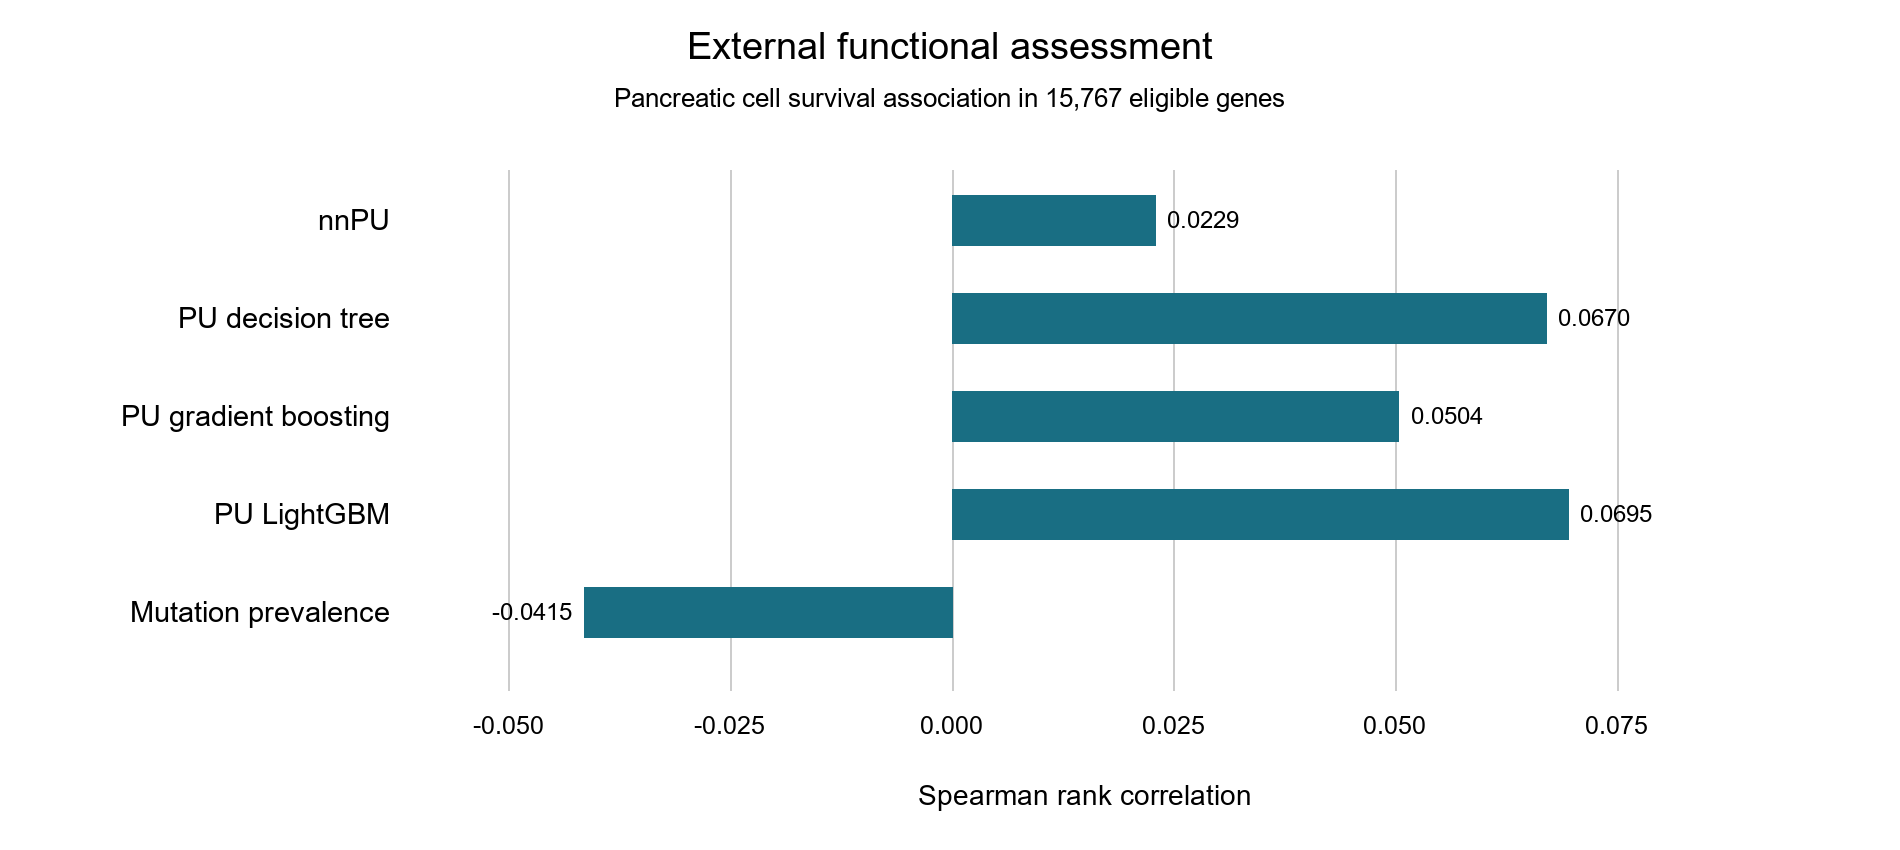
\includegraphics[width=\textwidth]{plot3.png}
\caption{Frozen-model functional assessment using Sanger Project Score. Survival dependency is distinct from driver status.}
\end{figure}
The CRISPR assessment uses Sanger Project Score data~\cite{ref15} and includes 15,767 eligible unlabelled, non-common-essential genes across 33 pancreatic adenocarcinoma donors, with 856 other-cancer donors for a specificity comparison. PANC-1 and its donor-related KP-1N model are excluded; related models are collapsed by donor. Model predictions remain frozen during external assessment.

Primary rank correlations are 0.0229 for nnPU, 0.0670 for the shallow tree, 0.0504 for gradient boosting and 0.0695 for LightGBM. These are small effects. None of the shortlisted models has top-100 enrichment against random gene sets, and pancreatic specificity is weak. The tree's nominal top-500 set expands to 1,684 genes because of score ties.

A survival knockout endpoint does not cover all driver mechanisms. Loss-of-function tumour suppressors need not appear as survival dependencies, and a broadly essential gene is not necessarily pancreas-specific. The weak associations limit claims of functional support without proving every high-ranking candidate irrelevant.

\chapter{Discussion and Evaluation Scope}
\section{Main achievements}
GenoPred integrates 19,962 genes, ten biological features and ten missingness indicators in a reproducible positive-unlabelled pipeline. Linear, tree and graph procedures are compared using retained source records, model bundles and evaluation outputs.

Linear nnPU achieves mean observed-label AP of 0.5517, compared with 0.5025 for mutation prevalence: an absolute improvement of 0.0492, or approximately 9.8\% relative to the baseline AP. The improvement is positive in all five repeat means. Mean top-100 and top-500 recall are 78.4\% and 85.6\%, respectively. These are descriptive internal retrieval results, not diagnostic accuracy.

\section{Biological and methodological insights}
The independently tuned comparisons identify mutation plus expression as a strong compact feature set, with nnPU AP of 0.5428 and top-100 recall of 82.0\%. Full-feature nnPU provides the highest mean AP in the feature comparison. The study therefore offers practical evidence for choosing between ranking precision, candidate recovery and assay complexity.

Gene-level tests complement the aggregate results. Full nnPU retrieves 94.1\% top-500 credit across the leave-one-positive-out tests and has mean top-100 weighted Jaccard stability of 0.793 over positive-deletion fits. External genomic assessments provide additional candidate-retrieval evidence with dataset-dependent model rankings. These outputs support a useful research shortlist and a clear basis for follow-up experiments.

\section{Essential evaluation qualifications}
The 17 positives are incomplete evidence labels and the remaining genes are not verified negatives. Model-family screening makes the repeated analysis retrospective; gene-level folds do not establish generalization to new patient cohorts. External genomic annotation and donor independence remain unresolved, while CRISPR correlations are small and no shortlisted model shows top-100 enrichment. Consequently, the results support exploratory gene prioritization rather than confirmed novel-driver discovery or clinical use. Independent validation is the main next step.

\chapter{Conclusion and Future Work}
GenoPred provides a reproducible pipeline for pancreatic driver-gene prioritization using molecular features, conservative positive-unlabelled labels and reproducible model comparisons. Repeated nested gene-level evaluation favours linear nnPU by mean observed-label AP among the shortlisted procedures, while mutation prevalence accounts for most of the available signal. Separately tuned analyses show a modest full-feature AP increment and a competitive mutation-plus-expression alternative.

External computational evidence produces dataset-dependent model rankings, and functional survival support is weak. The results support exploratory candidate prioritization and methodological comparison. They do not establish novel driver discovery, clinical performance or completed transfer learning.

\section{Priorities for continuation}
The first priority is a genuinely new, prospectively locked validation design with documented donor independence and an endpoint appropriate to the biological claim. Previously examined internal and external outcomes should be retained as development evidence, not reused as untouched tests.

The second priority is gene-specific evidence adjudication, licensed variant annotation where required, and explicit reconciliation of source discrepancies. High-ranking candidates need independent experimental or carefully curated mechanistic support before being described as new drivers.

The third priority is targeted methodological improvement: gene-callability sensitivity, validated sex-aware CNV handling, assay-specific value analysis and independent cohort robustness. Transfer learning and additional graph or Hi-C models should be preregistered as separate studies with negative-transfer controls and comparison against the pancreatic model trained from scratch.

The contribution of the present B.Tech Project I is the completed, inspectable research baseline and its limitations. Preserving unfavourable and unstable results is necessary for a credible next stage.

\appendix
\chapter{Reproducibility and Artifact Record}
\section{Evidence underlying the report}
The numerical snapshot is 4 November 2026. The report brings together the project's molecular dataset, repeated evaluation, feature comparisons and external assessments. The artifact categories below identify the retained evidence supporting the study.

\begin{table}[H]\centering
\caption{Principal evidence and reconstruction artifacts.}
{\small
\begin{tabularx}{\textwidth}{@{}>{\raggedright\arraybackslash}X>{\raggedright\arraybackslash}X@{}}\toprule
\textbf{Artifact} & \textbf{Purpose}\\\midrule
docs/FINAL\_\allowbreak RESULTS.md & Main repeated comparison and external evidence interpretation\\
docs/FINAL\_\allowbreak EXTENSION\_\allowbreak RESULTS.md & Feature groups, LOPO, stability and prior sensitivity\\
Main numerical comparison files & Main numerical comparison\\
Nested evaluation artifacts & Nested folds, selections, models and out-of-fold scores\\
Feature and sensitivity artifacts & Feature summaries, LOPO results and candidate stability\\
External gene and variant evidence & MSK gene and variant provenance\\
Autopsy source and evaluation records & Reconciled autopsy sources and evaluation\\
Feature and sensitivity protocol & Protocol recorded before extension fitting\\
\bottomrule\end{tabularx}}
\end{table}
\section{Reconstruction and verification}
From the project environment, the principal scripts are scripts/final\_\allowbreak robustness.py, scripts/build\_\allowbreak final\_\allowbreak results.py, scripts/final\_\allowbreak extension.py and scripts/report\_\allowbreak final\_\allowbreak extension.py, each invoked with the project root as its argument. The test suite is run with python -m pytest -q. Recorded manifests should be checked before comparing regenerated outputs.

The final extension contains 180 independently tuned outer model/feature evaluations, 68 LOPO evaluations and 30 fixed-prior evaluations. All 248 saved bundles in the first two groups reproduce their evaluation predictions exactly. The recorded suite contains 64 passing tests. Labels, fitted models, source hashes and evaluation outputs are retained for reproducibility.

\section{Exploratory model benchmark}
The broad Stage 6 benchmark completed 55 registered experiments, a validation-selected rank ensemble and four reference procedures, producing 60 comparison rows. It evaluated 95 candidate settings with three fixed seeds and retained warnings, preprocessing choices and saved-model round trips. Its fixed test subset contains only three known positives.

\begin{table}[H]\centering
\caption{Exploratory observed-label AP on the 3,992-gene fixed test subset.}
{\small
\begin{tabularx}{\textwidth}{@{}>{\raggedright\arraybackslash}X>{\raggedright\arraybackslash}X>{\raggedright\arraybackslash}X@{}}\toprule
\textbf{Procedure} & \textbf{AP} & \textbf{Status}\\\midrule
Linear nnPU & 0.22465 & Exploratory fixed split\\
STRING diffusion & 0.08844 & Exploratory fixed split\\
Shallow PU tree screen & 0.66721 & Exploratory broad screen\\
PU gradient boosting screen & 0.55641 & Exploratory broad screen\\
PU LightGBM screen & 0.55627 & Exploratory broad screen\\
\bottomrule\end{tabularx}}
\end{table}
The fixed-split screen demonstrates that multiple PU learner families can retrieve the observed evidence labels. Because its test subset contains only three positives and is used within exploratory development, the repeated nested comparison in Chapter 5 is the primary performance summary. The two designs evaluate different fitted procedures and gene partitions.

\section{Report preparation and review}
This report was prepared with AI-assisted drafting and formatting from the retained GenoPred project records. The student should review the technical interpretation, references and authorship declaration before signing. The declaration and supervisor certificate are intentionally unsigned, as in the reference report.

\chapter{Data Processing and Verification}
\section{Molecular measurement procedures}
Mutation input is parsed as tab-separated data with required-column and tumour/case-identity checks. Each case contributes at most once to a gene's selected mutation count. Under the project consequence definition, mutation prevalence is nonzero for 3,525 genes; KRAS is 94/165 and TP53 is 90/165.

Promoter signals use uniquely mapped windows with length, orientation and interior-position checks. Unavailable or distorted mappings are marked missing. Paired accessibility libraries are combined within each of 40 patient identifiers before patient-level summary statistics are computed.

Copy-number gain and loss are defined relative to each tumour's autosomal modal baseline. Sex-chromosome values remain explicitly unavailable pending a validated sex-aware calculation. Missingness flags distinguish unavailable measurements from observed zero signal.

\section{Ranking and model verification}
Average precision groups equal scores at common thresholds. Top-k recall assigns fractional credit at tied boundaries, and displayed ranks use midranks. This ensures that evaluation does not depend on arbitrary gene-identifier ordering within a tie.

Model bundles retain the intercept, weights, ordered inputs, imputation, scaling and relevant graph settings. Reload verification reproduces saved predictions exactly. Held-out-data isolation, feature-group isolation, fold coverage and tie-budget tests support the integrity of the evaluation.

\section{Reproducible experimental record}
The project retains source hashes, configurations, fold assignments, inner selections, fitted models and gene-level predictions. These records allow each reported table to be traced to an explicit calculation. Software verification supports reproducibility; biological interpretation is assessed separately through evidence retrieval, functional comparisons and follow-up validation.

\clearpage
\renewcommand{\bibname}{References}
\addcontentsline{toc}{chapter}{References}
\begin{thebibliography}{9}
\small
\bibitem{ref10} Kiryo R, Niu G, du Plessis MC, Sugiyama M. Positive-Unlabeled Learning with Non-Negative Risk Estimator. Advances in Neural Information Processing Systems 30, 2017. \url{https://arxiv.org/abs/1703.00593}
\bibitem{ref11} Szklarczyk D et al. The STRING database in 2023: protein--protein association networks and functional enrichment analyses for any sequenced genome of interest. Nucleic Acids Research 51(D1), D638--D646, 2023. \url{https://doi.org/10.1093/nar/gkac1000}
\bibitem{ref12} NCBI Gene Expression Omnibus. Source accession GSE149103. \url{https://www.ncbi.nlm.nih.gov/geo/query/acc.cgi?acc=GSE149103}
\bibitem{ref13} NCBI Gene Expression Omnibus. Source accession GSE124229. \url{https://www.ncbi.nlm.nih.gov/geo/query/acc.cgi?acc=GSE124229}
\bibitem{ref14} National Cancer Institute. Genomic Data Commons, TCGA-PAAD project. \url{https://portal.gdc.cancer.gov/projects/TCGA-PAAD}
\bibitem{ref15} Sanger Cancer Dependency Map. Whole-genome CRISPR knockout dataset documentation. \url{https://depmap.sanger.ac.uk/documentation/datasets/wg-crispr-knockout/}
\end{thebibliography}
\end{document}
